\documentclass[10pt,spanish,a4paper,openany,notitlepage]{article}
\usepackage{etex}
%-------------------------------------Paquetes-----------------------------------------------------------------------
\usepackage[spanish,es-tabla]{babel}  	% Traduce los textos a castellano
\usepackage[utf8]{inputenc}	% Permite escribir directamente áéíóúñ
\usepackage{t1enc}            	% Agrega caracteres extendidos al font
\usepackage{amsmath} 		%Permite imprimir mas opciones matemáticas
\usepackage{graphicx}		%Permite agregar imagenes al informe
\usepackage{float} 		%Permite utilizar H para colocar las imagenes en un lugar especifico 
\usepackage{units}
\usepackage{circuitikz}
\usepackage{caption}
\usepackage{subcaption}
\usepackage{sidecap}
\usepackage{mathtools}
\usepackage{multirow} % Paquete para dividir las tablas en subtablas
\usepackage{booktabs} %estos 2 sirven para achicar la tabla
\usepackage{tabulary}
\usepackage{fancyhdr} % encabezado
\usepackage{textcomp} % para usar ° con el comando \textdegree
\usepackage{anysize}		%Permite modificar los margenes del documento
\usepackage{abstract} % paquete para el resumen del articulo
\usepackage{amssymb}
\usepackage{courier}
\usepackage{color}
\usepackage{listings}
\usepackage{pdfpages}


\definecolor{dkgreen}{rgb}{0,0.6,0}
\definecolor{gray}{rgb}{0.5,0.5,0.5}

\lstdefinelanguage
   [x64]{Assembler}     % add a "x64" dialect of Assembler
   [x86masm]{Assembler} % based on the "x86masm" dialect
   % with these extra keywords:
   	{
   	alsoletter={.\#},	
	morecomment=[l]{;},
    	morestring=[b]',
	morekeywords={[1],\#define,.org,main,ldi,rcall,ramend,_sfr_io_ADDR,spl,sph,
					lds,sts,clr,cpse,rjmp,cbi,sbi,cpi,breq,,ocr2,,eecr,eewe,eearh,
					eearl,eecr,eere,eedr,ddrb,portb,cpi,cp,brlo,breq,sbrs,sbis,lsr,
					brsh,sbrc,sbic,pinb,.byte,.section,.text,.data,.eeprom,.end,
					lo8,hi8,.global,\#include,r1,r2,r3,r4,r5,r6,r7,r8,r9,10,r11,r12,
					r13,r14,r15,r16,r17,r18,r19,r20,r21,r22,r23,r24,r25,r26,r27,
					r28,r29,r30,r31,r32,r33,r34}
  	} % etc.

\lstset{language=[x64]Assembler,
   keywordstyle=\bf\color{blue},
   commentstyle=\it\color{dkgreen},
   stringstyle=\color{gray},
   numbers=left,
   numberstyle=\tiny\color{black},
   stepnumber=2,
   numbersep=8pt,
   backgroundcolor=\color{white},
   tabsize=4,
   showspaces=false,
   showstringspaces=false,
   extendedchars=\true,
	inputencoding=utf8}

% todo lo que sigue es para poner links que se les pueda hacer click
\usepackage{xcolor}
\usepackage[normalem]{ulem}
\usepackage{hyperref}
\hypersetup{colorlinks,urlcolor=blue}

\makeatletter
\DeclareUrlCommand\ULurl@@{%
  \def\UrlFont{\ttfamily\color{blue}}%
  \def\UrlLeft{\uline\bgroup}%
  \def\UrlRight{\egroup}}
\def\ULurl@#1{\hyper@linkurl{\ULurl@@{#1}}{#1}}
\DeclareRobustCommand*\ULurl{\hyper@normalise\ULurl@}
\makeatother

%---------------------------------------Configuraciones de pagina----------------------------------------------
\marginsize{2.5cm}{2.5cm}{1cm}{1cm}

\pagestyle{fancy}
\fancyhf{}
\lhead{
66.09 - \textsc{Laboratorio de Microcomputadoras}\\ 
1\textsuperscript{er} Cuatrimestre de 2015
}
\rhead{
\includegraphics[width=3cm]{imagenes/FIUBA_ALTA.jpg}}
\rfoot{Página \thepage}

%---------------------------------------Definiciones propias---------------------------------------------------------
\newcommand{\oiint}{\displaystyle\bigcirc\!\!\!\!\!\!\!\!\int\!\!\!\!\!\int} %Integral doble cerrada

\DeclarePairedDelimiter\abs{\lvert}{\rvert}%
\DeclarePairedDelimiter\norm{\lVert}{\rVert}%
% Swap the definition of \abs* and \norm*, so that \abs
% and \norm resizes the size of the brackets, and the 
% starred version does not.
\makeatletter
\let\oldabs\abs
\def\abs{\@ifstar{\oldabs}{\oldabs*}}
%
\let\oldnorm\norm
\def\norm{\@ifstar{\oldnorm}{\oldnorm*}}
\makeatother
%--------------------------------------------------------------------------------------------------------------------------------


\makeatletter
\let\ps@plain\ps@fancy 
\makeatother

% lo siguiente es para borrar el titulo del resumen y que no ocupe espacio:
 \AtBeginDocument{%
 \renewcommand{\abstractname}{}%
 }
\renewcommand{\absnamepos}{empty} % originally center
 

\begin{document}

\tableofcontents
\newpage

\section{Objetivos}
Se diseñará e implementará una pulsera térmica que regulará la
temperatura corporal. Se utilizará un módulo termoeléctrico para enviar
variaciones de calor o frío a la muñeca del usuario para modificar
la percepción térmica del cuerpo.

Su función es generar pulsos de frío o calor, de manera de generar una sensación de 
confort para una persona en condiciones donde la temperatura es muy alta 
o muy baja respectivamente.
Está basado en el proyecto \emph{Wristify} \cite{embrlabs} ganador del concurso de intel 
\emph{Make It Wearable} \cite{Make It Wearable}.


\subsection{Especificaciones}

El dispositivo utilizará una celda Peltier para enviar pulsos de calor
o frío. De forma que se logre una diferencia de temperatura mayor a $0,4\, \unit{^oC/seg.}$
durante 5 segundos y durante los siguientes 10 segundos entrará
en estado de espera, para luego volver a iniciar el ciclo. 

Deberá contar con un sensor de temperatura para medir la temperatura ambiente
y analizar si deberá enviar o recibir calor.

Finalmente deberá controlar que se cumpla el ciclo en base a la corriente
que circulará por la celda Peltier.

\subsubsection{Componentes}

Deberá contar con los siguientes componentes:

\begin{itemize}
\item{Celda Peltier:} Generará los pulsos de calor en la muñeca del usuario.
\item{Circuito regulador de corriente:} Regulará la corriente suministrada
a la celda peltier.
\item{Disipador:} La celda Peltier contará con un disipador para evitar
fijar la temperatura de una de sus placas.
\item{Termistores:} Contará con dos termistores. Uno para medir la
temperatura ambiente y en base a esta decidir el modo de trabajo, frío
o calor. El segundo termistor medirá la temperatura del disipador conectado
a la celda Peltier para poder realizar una estimación de la temperatura
de la celda.
\item{Salida de puerto serie:} Servirá para poder monitorear en una 
computadora la temperatura de la placa.
\item{Fuente:} Suministrará la corriente necesaria a la celda Peltier y 
 proporcionará alimentación a todos los dispositivos utilizados.
\item{Interruptor:} Para poder invertir el estado de trabajo, de frío a calor 
y viceversa.
\item{Controlador:} Se utilizara un microcontrolador AVR. Es
el encargado de obtener las temperaturas de los termistores para definir
el modo de trabajo y autoregular la corriente de la celda Peltier mediante
el circuito regulador de corriente.
\end{itemize}

\subsection{Diagrama de Flujo}

\begin{figure}[H] %[h] para here [b] para bottom [t] para top [H]+float para aqui si o si
\begin{center}
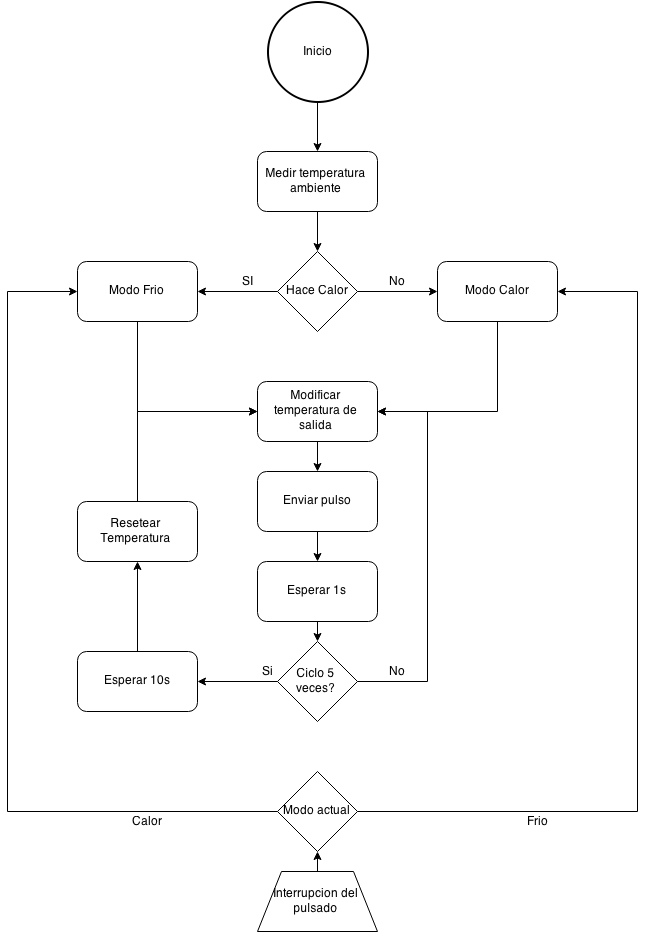
\includegraphics[scale=0.6]{./imagenes/diagrama_de_flujo.png}
\caption{Diagrama de flujo del proceso}
 \label{fig:diag_flujo}
\end{center}
\end{figure}

\subsection{Diagrama de Bloques}

\begin{figure}[H] %[h] para here [b] para bottom [t] para top [H]+float para aqui si o si
\begin{center}
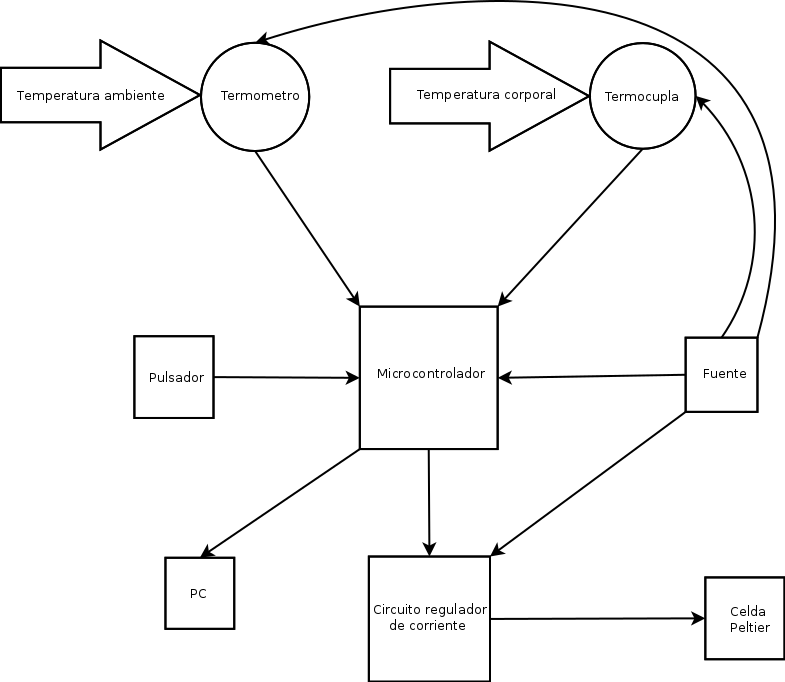
\includegraphics[scale=0.5]{./imagenes/diagrama_de_bloques.png}
\caption{Diagrama de bloques}
 \label{fig:diag_bloques}
\end{center}
\end{figure}


\section{Diseño}

\subsection{Esquematico}


\begin{figure}[H] %[h] para here [b] para bottom [t] para top [H]+float para aqui si o si
\begin{center}
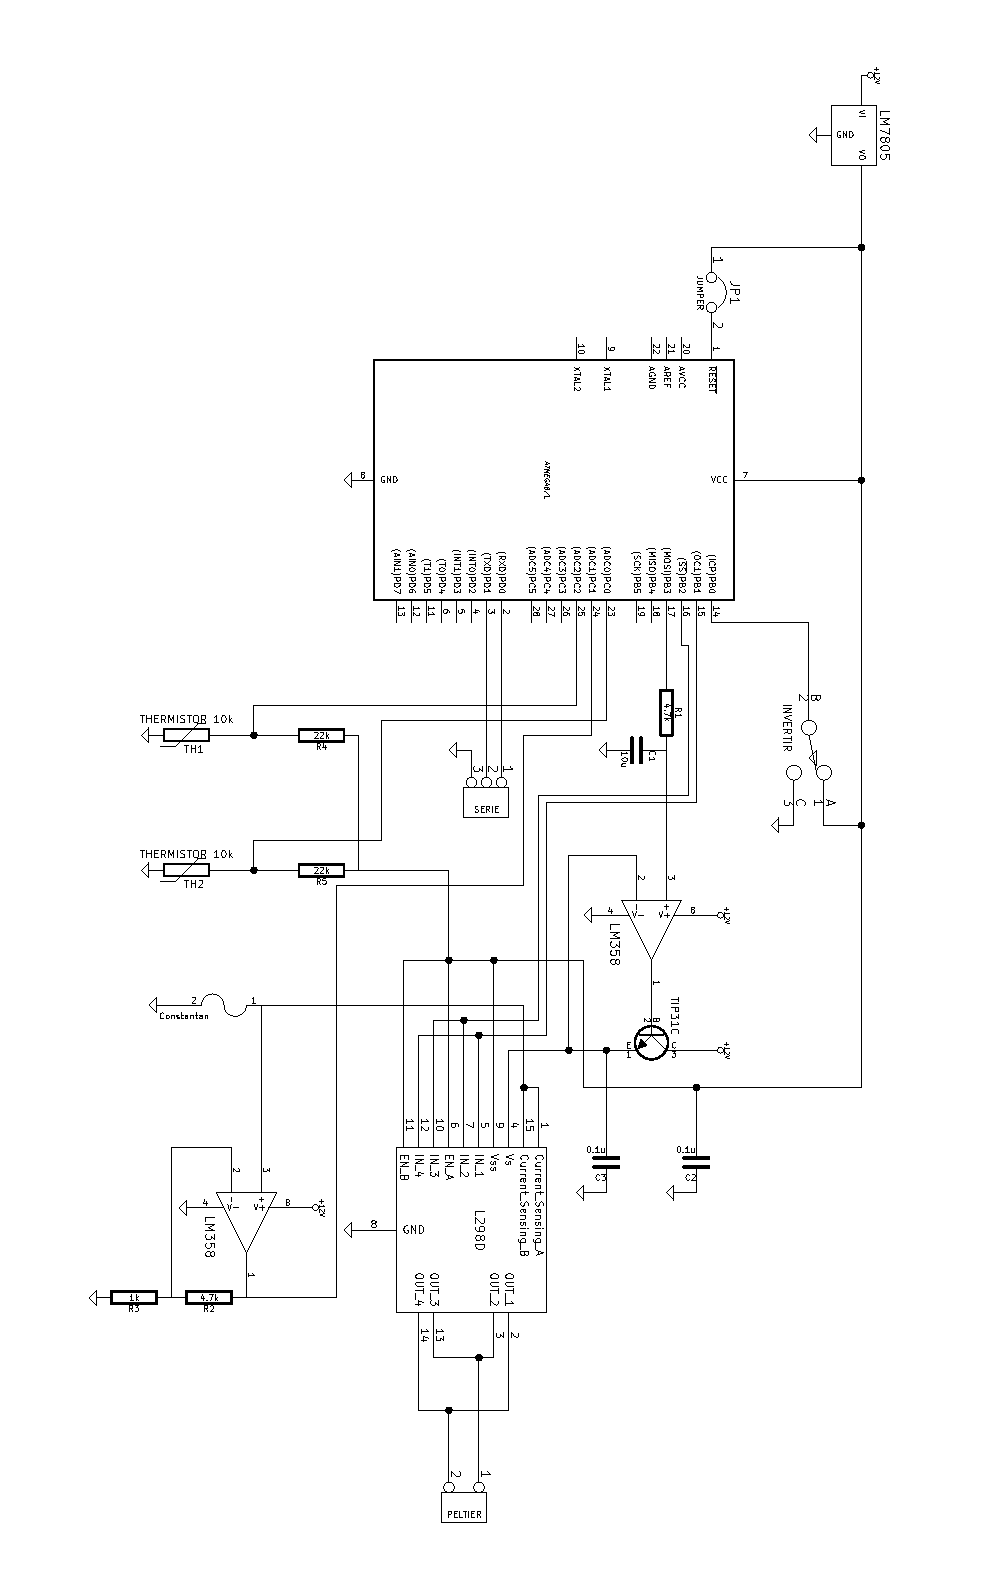
\includegraphics[scale=0.8]{../circuitos/esquematico.pdf}
\caption{diagrama esquemático}
 \label{fig:esquematico}
\end{center}
\end{figure}

\subsection{Componentes}

\begin{itemize}
\item{Celda Peltier:} Celda peltier de $10\, \unit{W}$ y $15\, \unit{mm}$x$15\,\unit{mm}$ 
\item{LM7805:} Regulador de tensión para habilitar el puente H, alimentar
el microcontrolador y suministrarle tensión constante a las resistencias conectadas
en serie a los termistores.
\item{Interruptor:} Interruptor para activar la inversión de la polaridad.
\item{Resistencias:}
	\begin{itemize}
	\item Dos resiststencias de $4.7\,\unit{k\Omega}$
	\item Dos resiststencias de $22.0\,\unit{k\Omega}$
	\item Una resistencia de $1.0\,\unit{k\Omega}$
	\end{itemize}
\item{Capacitores:} 
	\begin{itemize}
	\item 1 capacitor de \unit{10\, \unit{$\mu$F}} para generar
	tensión constante del PWM recibido.
	\item 2 capacitores de \unit{0.1\, \unit{$\mu$F}} Conectados en paralelo
	a las alimentaciones del puente H, recomendados por el fabricante. 
	\end{itemize}
\item{LM358:} Dos amplificadores operacionales. Uno para suministrar corriente
a la base del NPN y el segundo para amplificar la tensión leída del constantán. 
\item{TIP31C:} Transistor de potencia NPN, utilizado para regular la corriente.
\item{L298D:} Puente H utilizado para invertir la polaridad de la celda Peltier
\item{Constantán:} alambre utilizado para sensar la corriente generada.
\item{Bateria:} de $12\, \unit{V}$ y $2.9\, \unit{Ah}$
\item{Pines:}
	\begin{itemize}
	\item 3 pines para el puerto serie.
	\item 2 pines para el reseteo del microcontrolador.
	\item 2 pines para conectar la celda peltier al circuito.
	\end{itemize}
\item{Termistores:} Dos termistores NTC de $10\, \unit{k\Omega}$
\end{itemize}

\subsection{Regulador de Corriente}

Se utilizó un regulador de corriente controlado por un PWM como se muestra
en la figura \ref{fig:reg_corriente}

\begin{figure}[H] %[h] para here [b] para bottom [t] para top [H]+float para aqui si o si
\begin{center}
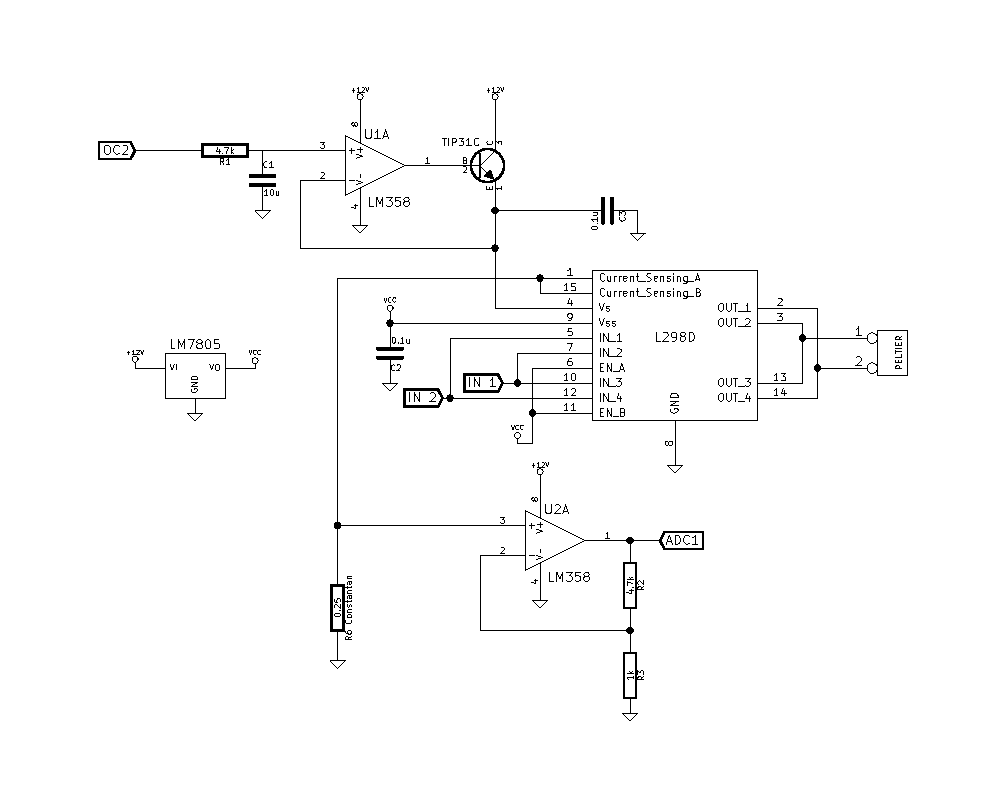
\includegraphics[scale=0.75]{../circuitos/regulador_corriente.pdf}
\caption{Regulador de Corriente}
 \label{fig:reg_corriente}
\end{center}
\end{figure}

El circuito RC generará una tensión constante del PWM generado por el
microcontrolador. Dicha tensión regulará la corriente suministrada a la
base del NPN por el amplificador operacional, generando una corriente
constnte entre el colector y el emisor del transistor.

Se optó por utilizar un L298D para el puente H ya que cuenta en un mismo
integrado dos puentes H que soportan $2\, \unit{A}$ de corriente. 
Conectados en paralelo como se muestra en la figura \ref{fig:reg_corriente} 
se puede duplicar dicha corriente máxima para que soporte hasta $4\, \unit{A}$ de corriente.

Al final del circuito se sensará la corriente generada mediante la tensión
en el alambre constatán que es amplificada por el amplificador operacional.
Para que la tensión de salida varíe entre $0\, \unit{V}$ y $2.56\, \unit{V}$
y sea leído por el microcontrolador.

Las resistencias del amplificador se obtuvieron considerando que para
la corriente maxima registrada, la salida no supere los $2.56\, \unit{V}$.
Se registró una corriente maxima de $1.75\, \unit{A}$ y se midió una
resistencia de $0.25\, \unit{\Omega}$.

La tensión de salida se obtiene mediante:

\begin{equation}
V_{ADC1} = R_{constantan} I_{MAX} \frac{R_3 + R_2}{R_3}
\label{eq:tension_salida}
\end{equation}

Luego fijando $R_3 = 1\, \unit{k\Omega}$ y $R_2 = 4.7\, \unit{k\Omega}$
se verificó que la tensión no supere los $2.56\, \unit{V}$:

\[ \displaystyle V_{ADC1} = 0.25\, \unit{\Omega}\ 1.75\, \unit{A} \frac{1\, \unit{k\Omega} + 4.7\, \unit{k\Omega}}{1\, \unit{k\Omega}} = 2.49 \unit{V} \]

\subsection{Medición de la temperatura}

Para medir la temperatura se utilizó un divisor resistivo
utilizando termistores para medir su tensión y poder estimar la temperatura.
Se obtuvieron las resistencias a conectar en serie con los termistores de
forma que la tensión maxima no supere los $2.56\, \unit{V}$

\begin{figure}[H] %[h] para here [b] para bottom [t] para top [H]+float para aqui si o si
\begin{center}
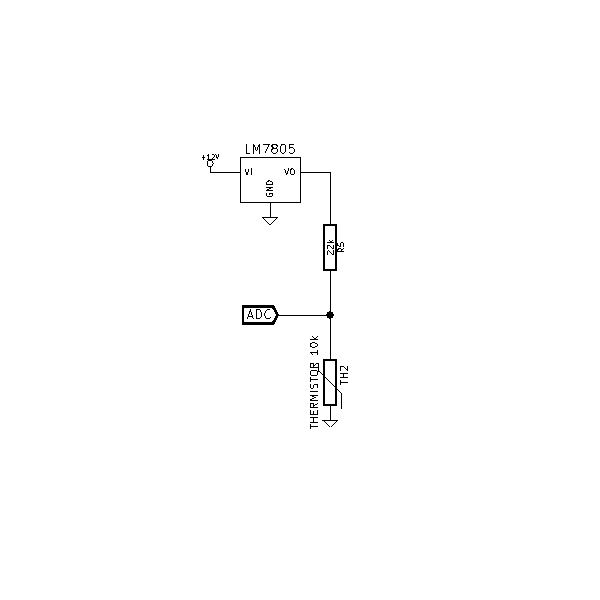
\includegraphics[scale=1]{../circuitos/temperatura.pdf}
\caption{Divisor de tensión de los termistores}
 \label{fig:temperatura}
\end{center}
\end{figure}

\begin{equation}
V_{termistor} = 5\, \unit{V} \frac{R_{termistor}}{R_{termistor}+R_{serie}}
\label{eq:tension_termistor}
\end{equation}

Finalmente se eligió una resistencia de $R_{serie} = 22\, \unit{k\Omega}$
para $R_4$ y $R_5$ verificando que la tensión en los termistores no supere
la tensión de referencia del ADC del microcontrolador para la resistencia
maxima registrada en los termistores a $R_{0\,\unit{^oC}} = 15\, \unit{k\Omega}$ :

\[ \displaystyle V_{termistor} = 5\, \unit{V} \frac{15\, \unit{k\Omega}}{15\, \unit{k\Omega}+22\, \unit{k\Omega}} = 2\, \unit{V}\]

\section{Especificaciones del microcontrolador}

\subsection{Microcontrolador}
Para este proyecto se utilizo un microcontrolador \texttt{Atmega8L}. El datasheet del mismo se puede obtener en la pagina de Atmel\cite{datasheet}
\subsection{Configuraciones}
\subsubsection{Low Fuse}
Se configuro este registro para que el clock del microcontrolador estuvise establecido en 8MHz. 
\begin{center}
\begin{tabular}{|c|c|c|c|c|c|c|c|}\hline
7&6&5&4&3&2&1&0\\\hline
\textbf{1}&\textbf{1}&\textbf{1}&\textbf{0}&\textbf{0}&\textbf{1}&\textbf{0}&\textbf{0}\\\hline
BODLVL&BODEN&SUT1&SUT0&CKSEL3&CKSEL2&CKSEL1&CKSEL0\\\hline
\end{tabular}
\end{center}
Solo se modificaron los valores de CKSEL, el resto de los bits fue dejado en la configuracion que venia de fabrica.

\subsubsection{UCSRC}\label{UCSRC}
Se configuro este registro para setear que el puerto serie envie datos de 8bits, con un bit de stop y sin bit de paridad
\begin{center}
\begin{tabular}{|c|c|c|c|c|c|c|c|}\hline
7&6&5&4&3&2&1&0\\\hline
\textbf{1}&\textbf{0}&\textbf{0}&\textbf{0}&\textbf{0}&\textbf{1}&\textbf{1}&\textbf{0}\\\hline
URSEL&UMSEL&UPM1&UPM0&USBS&UCSZ1&UCSZ0&UCPOL\\\hline
\end{tabular}
\end{center}

\begin{description}
\item{Configuracion segun el bit}
\item{Bit 7}:
\item{Bit 6}: Modo Asincronico
\item{Bit 5 y 4}: Sin bit de paridad
\item{Bit 3}: Un bit de STOP
\item{Bit 2 y 1}: Datos de 8 bits
\item{Bit 0}: 0 Por modo Asincronico
\end{description}

\subsubsection{UBRRL}
Se configuro este registro para setear el Baud Rate del puerto serie a $38.4Mhz$
\begin{center}
\begin{tabular}{|c|c|c|c|c|c|c|c|}\hline
7&6&5&4&3&2&1&0\\\hline
\textbf{0}&\textbf{0}&\textbf{0}&\textbf{0}&\textbf{1}&\textbf{1}&\textbf{0}&\textbf{0}\\\hline
\multicolumn{8}{|c|}{UBRR[7:0]}\\\hline
\end{tabular}
\end{center}

\subsubsection{TCCR2}\label{TCCR2}
Se configuro este registro para setear el modo de funcionamiento del contador 2. 
\begin{center}
\begin{tabular}{|c|c|c|c|c|c|c|c|}\hline
7&6&5&4&3&2&1&0\\\hline
\textbf{0}&\textbf{1}&\textbf{1}&\textbf{1}&\textbf{0}&\textbf{0}&\textbf{0}&\textbf{1}\\\hline
FOC2&WGM20&COM21&COM20&WGM21&CS22&CS21&CS20\\\hline
\end{tabular}
\end{center}

\begin{description}
\item{Configuracion segun el bit}
\item{Bit 7}: 0, por ser modo PWM
\item{Bit 6 y 3}: Modo PWM, Phase Correct
\item{Bit 5 y 4}: Modo set on match en subida y clear on match en bajada
\item{Bit 2 - 0}: Sin prescaler
\end{description}

\section{Software}

\subsection{Protocolo puerto serie}
Para la comunicacion desde el puerto serie se utilizo un protocolo con el siguiente formato:

\begin{itemize}
\item \textbf{Primer bloque}: Un byte con un caracter \textit{ASCII} alfanumerico identificador el dato a mandar.
\item \textbf{Siguientes bloque}: Uno o mas bytes con el dato a enviar. El receptor se debe encargar de determinar el largo de este en base a lo recibido en el primer bloque.
\end{itemize}

En particular para este proyecto, se utilizaron datos de un byte\footnote{Esto fue en parte una consecuencia de la eleccion del modelo del microcontrolador. Por otro lado, tampoco eran necesarios datos mas grandes.} y se enviaron con la configuracion detallada en la seccion \ref{UCSRC} (Pagina: \pageref{UCSRC}), con lo cual los paquetes enviados por puerto respetan el siguiente formato:

\begin{center}
\begin{tabular}{|c|c|c|c|c|c|}\hline
1-bit&8-bits&1-bit&1-bit&8-bits&1-bit\\\hline
START&Tipo de dato&STOP&START&Dato enviado&STOP\\\hline
\end{tabular}
\end{center}


\section{Conclusiones}

En este punto se hará una autocrítica acerca de los errores y aciertos 
logrados . También se podrán  hacer sugerencias sobre futuras mejoras 
en el proyecto y si consideran que otro grupo lo puede continuar. Incluir 
en este punto las diferencias, si las hubiere, entre las especificaciones 
originales previstas en el anteproyecto y las finalmente alcanzadas.


Las celdas Peltier son dispositivos muy delicados, por lo que requerirá
estar bien protegidas a posibles impactos, ya que el mínimo impacto
las daña permanentemente. 
No se logró encontrar una relación simple entre la corriente de la celda
y su diferencia de temperatura, ya que esta no solo depende de la corriente
sino también de la temperatura inicial. Por los datos medidos para realizar
las tablas llegamos a la conclución de que la corriente fija una velocidad
a la que la temperatura variará hasta llegar a un valor pico.

Fué mas facil regular el modo frío ya que al iniciar el standby la
temperatura regresaba rapidamente a su valor inicial. En cambio para el
modo calor, al iniciar el standby la celda peltier no llega a enfriarse
hasta obtener su valor inicial luego del standby, por lo que en cada ciclo
irá acumulando temperatura hasta llegar a un valor máximo que depende
de la corriente máxima que reciba.

Por las mismas razones mencionadas sobre el comportamiento de la celda Peltier,
deducir su temperatura en base a la temperatura del disipador y la corriente
que circula por la celda devuelve datos poco presisos, lo que se podria calcular
es la diferencia de temperatura entre cada pulso con el inicio del ciclo.
Para medir la temperatura del peltier se deberá agregar una placa que
transmita el calor del peltier para aumentar su superficie y poder medir su
temperatura directamente con una termocupla, ya que detectan mas rápido
los cambios bruscos de temperatura, a diferencia de los termistores. 


Finalmente, para lograr las condiciones especificadas por el proyecto
no es necesario generar corrientes altas. Con una corriente máxima de
$500\, \unit{mA}$ bien reguladas se hubiese logrado el objetivo del producto
y se habría reducido su tamaño debido a que no requiere una batería de
gran tamaño.

\appendix 

\newpage
\section{Codigo Proyecto}
\subsection{Pulsera.S}
\lstinputlisting{../codigo_proyecto/pulsera.S}
\newpage
\lstset{language=Make}
\subsection{Makefile}
\lstinputlisting{../codigo_proyecto/Makefile}

\section{Datasheets}

\includepdf[pages={1-2}]{../datasheet/Atmega8L.pdf}

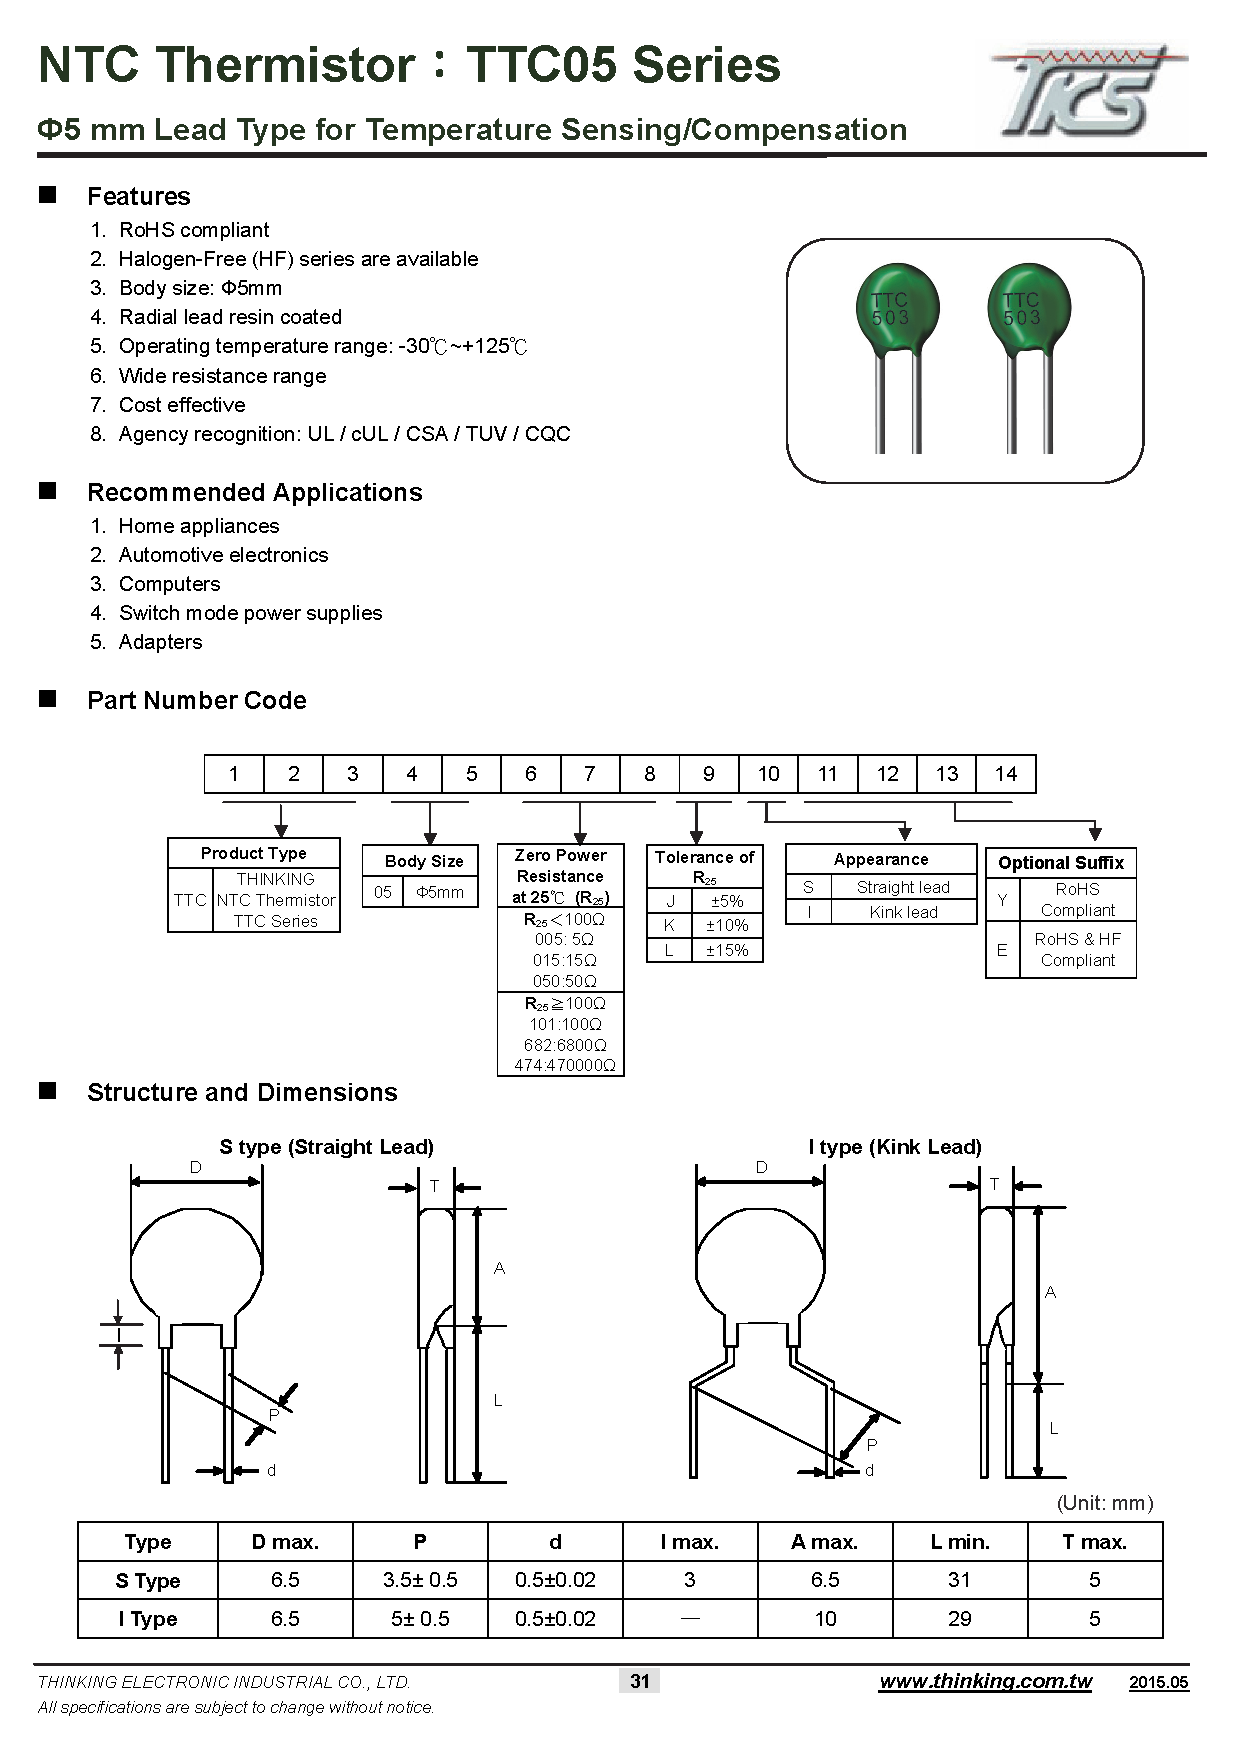
\includepdf[pages={1-8}]{../datasheet/termistor.pdf}

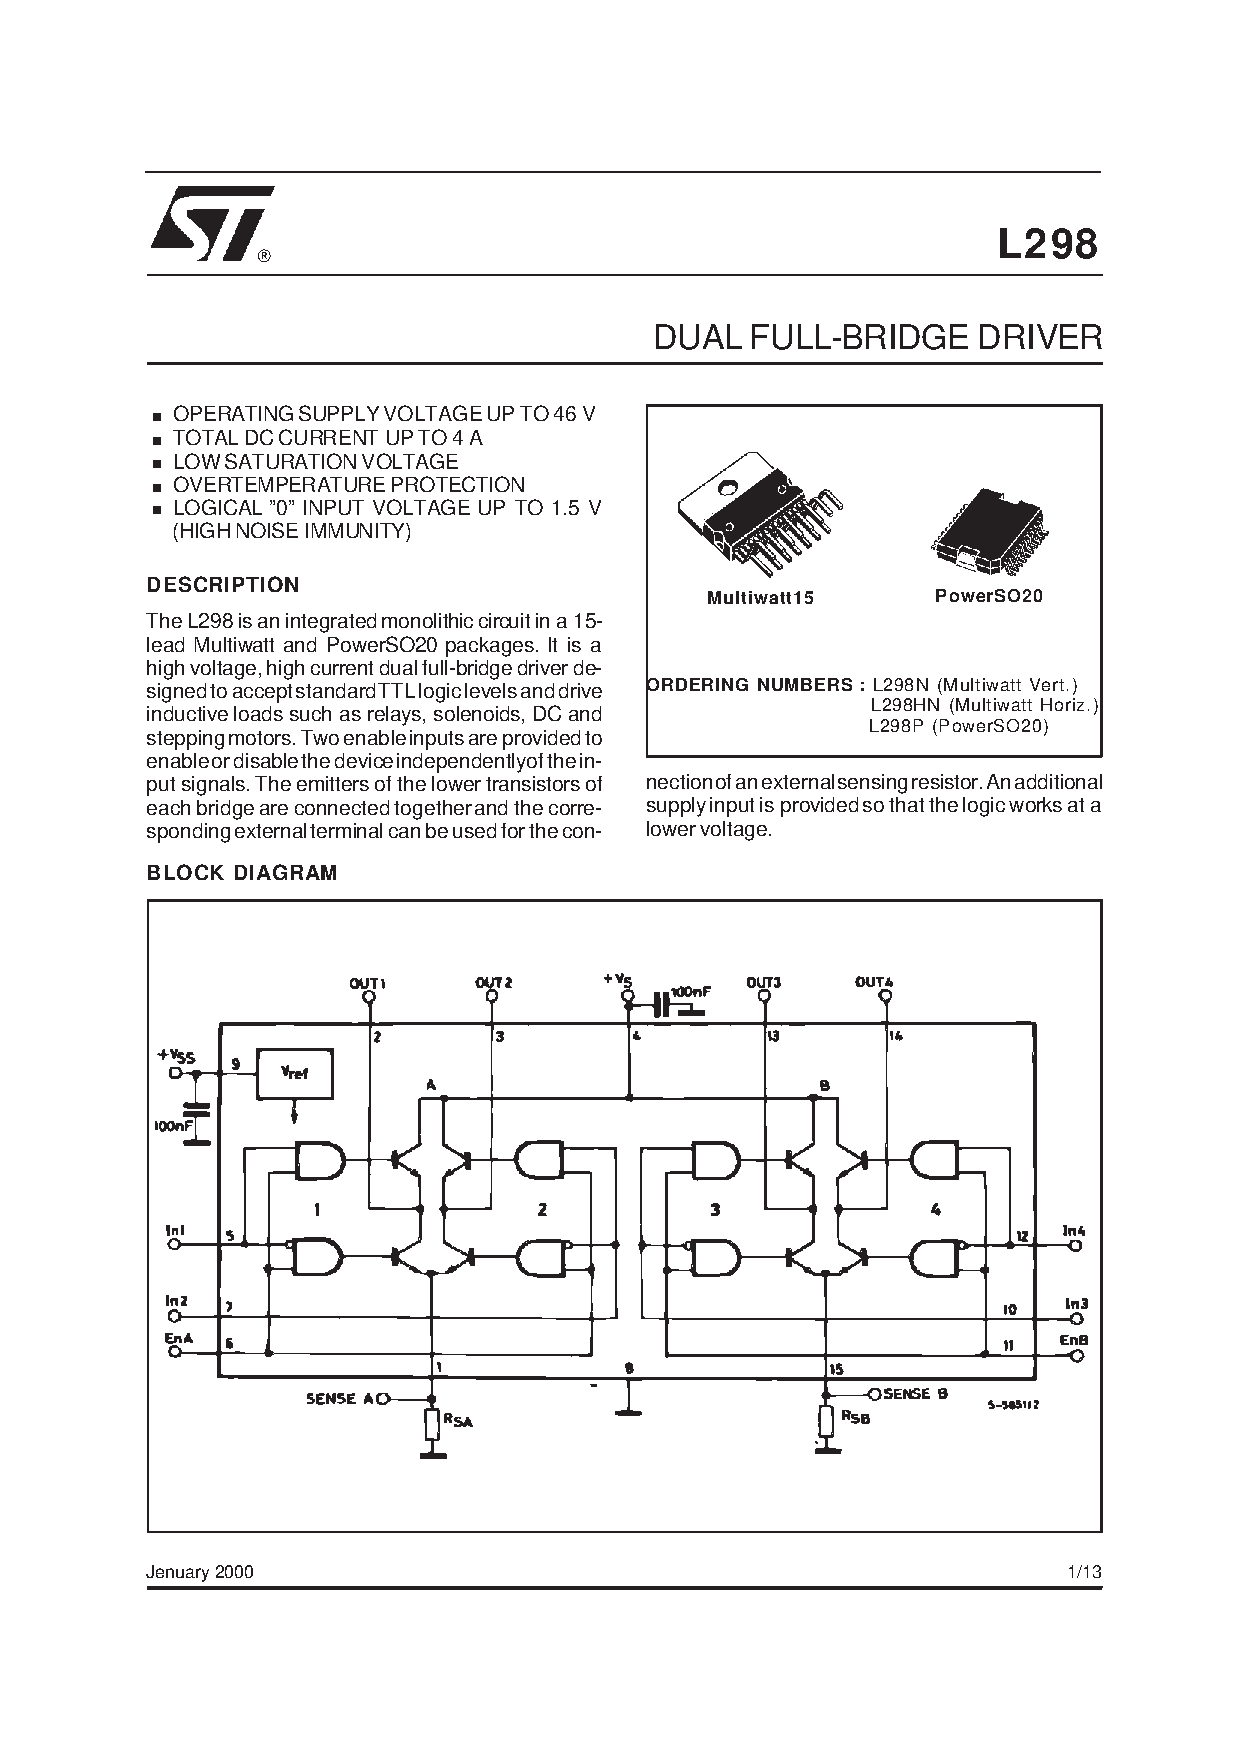
\includepdf{../datasheet/L298.pdf}

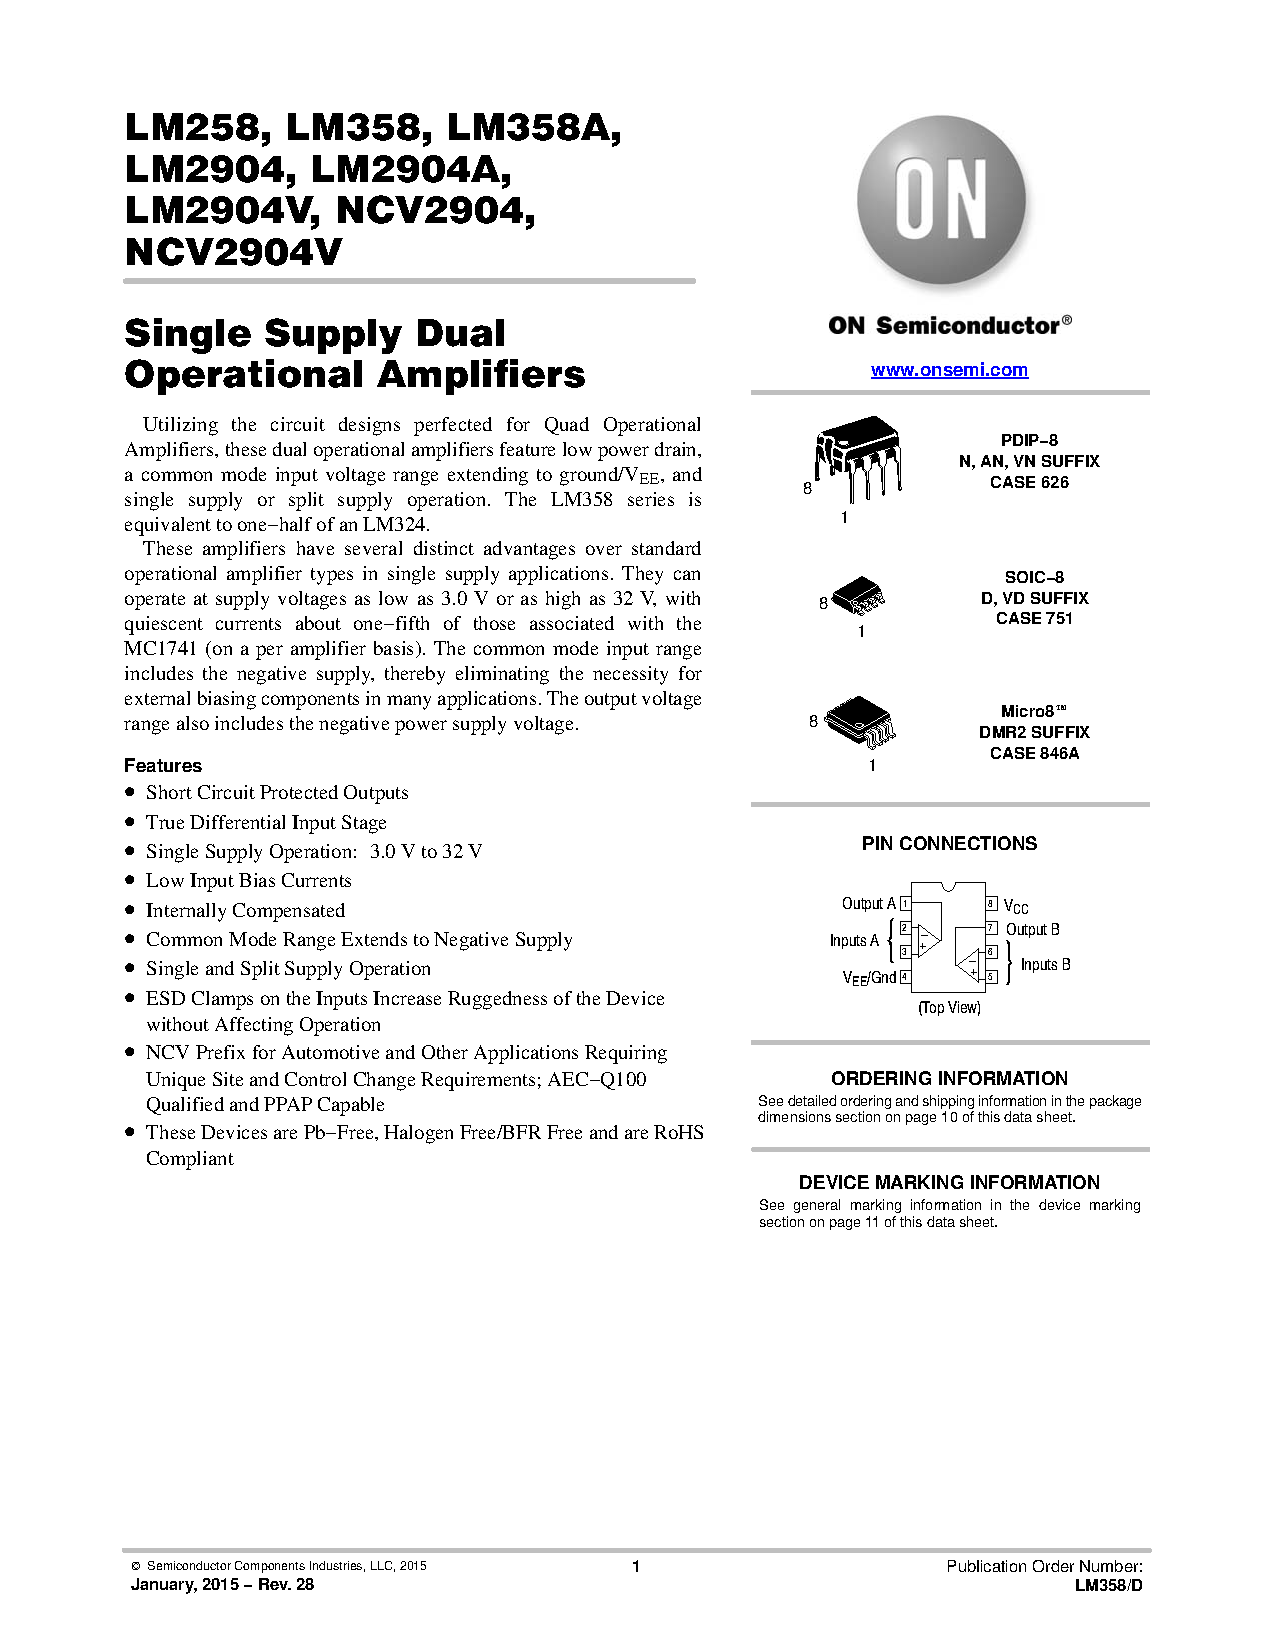
\includepdf{../datasheet/LM358.PDF}

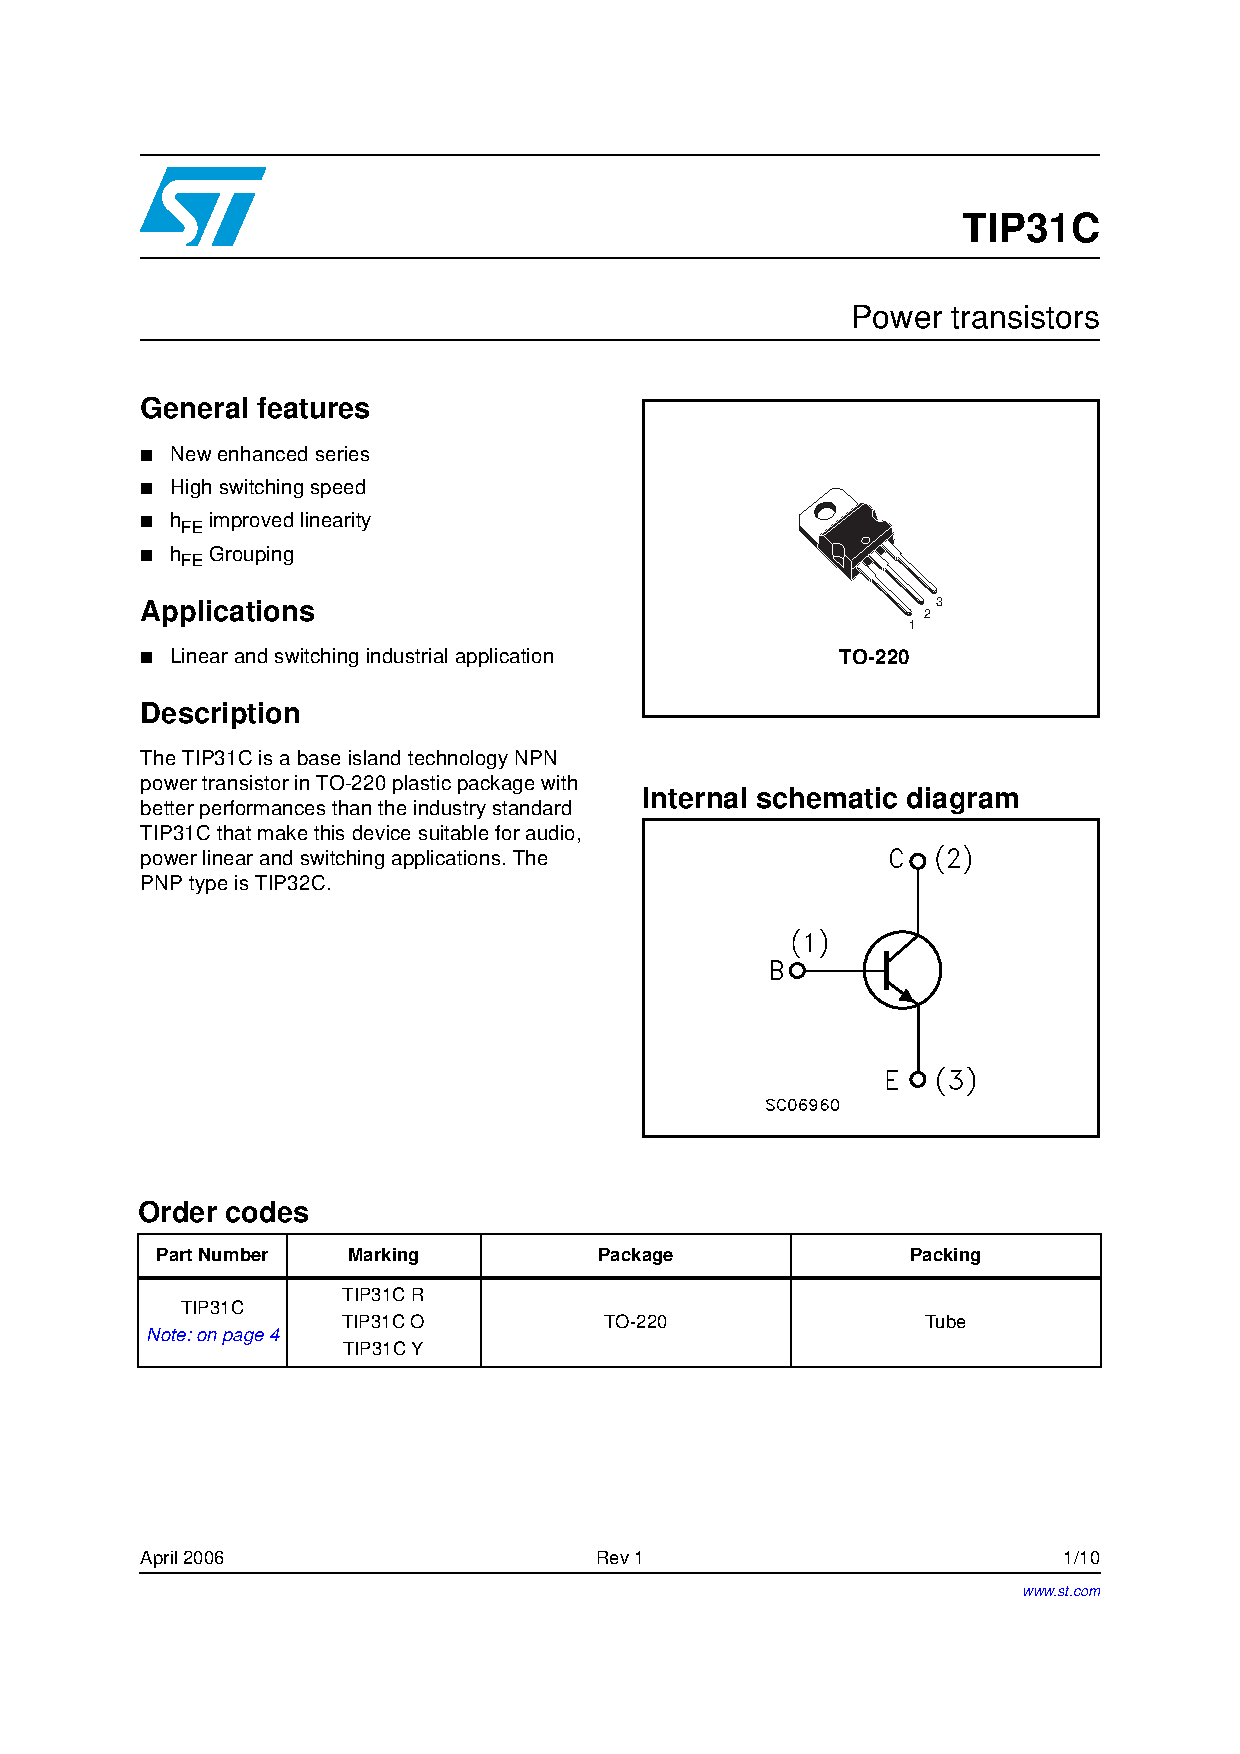
\includepdf{../datasheet/TIP31C.pdf}

\newpage
\section{Referencias}
\begin{thebibliography}{9}

\bibitem{embrlabs}
  \ULurl{http://www.embrlabs.com/}

\bibitem{Make It Wearable}
  \ULurl{https://youtu.be/sDZHITVfYrI}
  
\bibitem{video MIT}
  \ULurl{https://youtu.be/kvUMCip-r4A}

\bibitem{datasheet}
  \ULurl{http://www.atmel.com/images/atmel-2486-8-bit-avr-microcontroller-atmega8_l_datasheet.pdf}

\end{thebibliography}

\newpage
\section{Presupuesto}

\begin{center}
\begin{tabular}{|l|r|r|r|}\hline
Componente&Precio xU&Cantidad&Precio total\\ \hline
Celda Peltier $10\, \unit{W}$ $15\, \unit{mm}$x$15\, \unit{mm}$ &\$120.00&1&\$120.00\\ \hline
Atmega8-L &\$42.00&1&\$42.00\\ \hline
L298 &\$47.00&1&\$47.00\\ \hline
LM358 &\$8.00&1&\$8.00\\ \hline
LM7850 &\$5.00&1&\$5.00\\ \hline
Disipador &\$10.00&3&\$36.00\\ \hline
Termistor &\$7.00&2&\$14.00\\ \hline
Resistencia &\$0.5&5&\$2.50\\ \hline
Capacitor &\$0.50&3&\$1.50\\ \hline 
Bateria &\$160.00&1&\$160.00\\ \hline
Interruptor &\$5.00&1&\$5.00\\ \hline
Placa perforada &\$26.00&1&\$5.00\\ \hline
\multicolumn{3}{|r|}{Total}&\$467.00\\ \hline
\end{tabular}
\end{center}

\end{document}
